\chapter{Obesity associated genetic signatures and pathway signatures}
\label{cha:obesity_associated_genetic_signature_and_pathway_signatures}

In this chapter, the underlying biological mechanism of the obesity associated signatures from Creighton's data were investigated.
In doing so, Gatza's pathway genetic signatures were utilised to determine which biological pathways the obesity associated genetic signatures were most similar to.
First, the direction of Gatza's pathway associated genetic signatures were resolved; then the pathway associated metagenes were compared with the obesity associated metagenes; and lastly linear models were constructed based on the pathway metagenes and sample \gls{bmi}/\gls{bmi} status to predict the obesity associated metagenes.

\section{Pathway associated genetic signatures from \citet{Gatza2010a} study}
\label{sec:pathway_associated_genetic_signatures_from_gatza2010a_study}

Pathway associated genetic signatures from the \citet{Gatza2010a} study were examined for their consistency with the reported results.
In the \citet{Gatza2010a} study, their data comprised of samples from different data sets from other studies, \gls{mas}-normalised and the metagene scores were ranked with probit.
However, the analyses so far have used \gls{rma}-normalisation method and ranked based on the number of samples present in the data.
To decide which normalisation or ranking methods were suitable for the analysis, the different methods were compared in Gatza's data (see \cref{app:b}).
Results shown in \cref{app:b} clarified that there was no significant difference in the ranking methods used.
Correlation and scatter plots of the different combinations of transformation matrices (derived from either \gls{rma}- or \gls{mas}-normalised data) with \gls{rma}- or \gls{mas}-normalised data.
It seemed like the normalisation methods of the data in which the transformation matrices were applied to had the most significant effect on the resulting metagenes, rather than the transformation matrices themselves (\cref{app:b}).
This meant that all of the data sets had to be normalised with a single normalisation method, so \gls{rma} normalisation method was used as this method was more reliable than the \gls{mas} method.
Therefore, Gatza's data set was batch corrected first (\cref{sub:batch_correction}), then normalised with \gls{rma} method and the scores were ranked based on the number of samples in the data set.

One thing to be noted from these scatter plots was that there were some pathway signatures that were more variable than the others.
As an example, the \gls{tgfb} metagenes were significantly more dispersed compared to the \gls{pr} metagenes, even though these metagenes were both generated similarly in the same data set (add figure).
These differences were seen in other data sets as well (\cref{app:b}).
This result provided evidence that some of the pathway genetic signatures from the \citet{Gatza2010a} study were more consistent across different data sets than the others.
\\

\noindent
Before Gatza's pathway metagenes were compared with the obesity associated metagenes, the direction of Gatza's pathway metagenes had to be checked to make sure the metagenes were in the correct direction (\cref{sub:metagene_direction}).
% Each pathway metagenes was generated from Gatza's data set and the direction of the metagene was checked with the expression of the representative pathway gene (\cref{tab:metagene_direction}), and the groupings of the pathways were considered as well.
The correlation of all the pathway metagenes with one another were plotted as a heatmap in \cref{fig:gatza_meta_dir}.
The most prominent group had five pathways (E2F1, \gls{pi3k}, Myc, \gls{bcat} and Ras) that clustered at the top right hand corner of the heatmap.
% TODO: add additional info about why these pathways clustered together?
Other groups included \gls{ifna}/\gls{ifny}/\gls{tnfa} pathways, \gls{er}/\gls{pr}/p53 pathway and p63/\gls{her2} pathways.
In addition to these highly correlated groups, \gls{stat3}/\gls{tgfb}/Src/\gls{egfr}/Akt pathways showed little correlation with one another.
Comparing these groups with the results presented by \citet{Gatza2010a} (see \cref{app:b}), the identified groups approximately resembled the groups identified in their study, which confirmed that the directions of Gatza's pathway metagenes were similar to those used in the \citet{Gatza2010a} study.

\begin{figure}[htpb]
	\centering
	\includegraphics[page=15,width=0.7\linewidth]{results2/gatza_meta_trans}
	\caption{Gatza metagene direction}
	\label{fig:gatza_meta_dir}
\end{figure}

To see whether the directionality of Gatza's pathway metagenes were being transferred across to other data sets properly, pathway metagenes were generated in other data sets with the transformation matrices and the groupings of the metagenes were examined.
Creighton's, FM's and Cris' data were \gls{rma}-normalised and transformation matrices of the pathway genetic signatures (derived from Gatza's data set) were applied to the data sets.
The metagenes were plotted in a heatmap (shown in \cref{app:b}), which showed similar groupings  as seen in \cref{fig:gatza_meta_dir}.
This result confirmed that the pathway metagenes were acting similarly in all the data sets in which the transformation matrices have been applied to.

% In order to investigate what the underlying biological mechanism of the obesity associated genetic signatures was, Gatza's pathway associated genetic signatures were used to create linear models to predict the obesity associated metagene scores.
% Before linear models were created, Gatza's pathway metagenes were checked for their directionality to ensure that the pathway metagenes were acting as reported by \citet{Gatza2010a} (see \cref{sub:metagene_direction}).

\section{Pathway associated metagenes and obesity associated metagenes}
\label{sec:pathway_associated_metagenes_and_obesity_associated_metagenes}

Results from previous section confirmed that the pathway metagenes from the \citet{Gatza2010a} study were in the correct directions, and that the pathway metagenes were behaving as expected in different data sets.
Now that the directions of the pathway metagenes were established, these metagenes were ready for comparison with the obesity associted metagenes.
However, all of the pathway metagenes were derived from Gatza's data, whereas the majority of the obesity associted metagenes were derived from Creighton's data, which presents a problem of deciding on which data set the transformation matrices should be generated in.

In theory, the metagenes generated from the application of \gls{svd} and the metagenes generated from transformation matrix would be exactly the same if the transformation matrix was derived from the same data set.
For example, an obesity associted metagene generated from Creighton's data with \gls{svd} would have the same values as the metagenes generated in Creighton's data with the transformation matrix (where the transformation matrix was derived from Creighton's data).
Furthermore, if the \gls{svd}-derived metagenes and transformation matrix-derived metagenes were the same (or at least similar) in a different data set, this suggests that there was no difference in the data sets, at least in terms of the expression of the genetic signatures being investigated.
In other words, the transformation matrix can be made in either the original data set or in a different data set, if there is no difference in the \gls{svd}-derived or transformation matrix-derived metagenes.

% TODO: start from here
To decide which data set the transformation matrices for obesity and pathway associated genetic signatures should be generated in, the \gls{svd}- and transformation matrix(TM)-generated metagene scores were compared in all of the data sets.
As in \cref{sec:pathway_associated_genetic_signatures_from_gatza2010a_study}, all data sets were normalised with the \gls{rma} method and metagenes were ranked based on the number of samples in each data set.
Transformation matrices for the obesity associted genetic signatures were made in Creighton's data set and pathway associted genetic signatures were made in Gatza's data set.
Metagenes for all of the obesity and pathway associated genetic signatures were generated in all of the data sets with \gls{svd} and transformation matrices.
The Spearman correlation of the \gls{svd}-generated and TM-generated metagene scores were calculated for each genetic signatures.

\begin{table}[htpb]
	\centering
	\caption{Spearman correlation of the svd vs tm metagenes}
	\label{tab:svd_vs_tm}
	\begin{tabular}{c}
		gtrmatransres (RMA)
		\hline
		FM & Creighton   &     Cris
		akt   -0.5563 -0.5190 -0.5900
		bcat   0.9905  0.9897  0.9977
		e2f1   0.9193  0.9646  0.8438
		egfr  -0.4040 -0.0430 -0.3358
		er     0.9966  0.9978  0.9942
		her2  -0.9794 -0.9553 -0.5817
		ifna   0.9951 -0.9830 -0.9991
		ifng   0.9718 -0.9086  0.9950
		myc    0.9689  0.9878 -0.9852
		p53    0.7923  0.3808  0.9981
		p63    0.8368  0.8319  0.2951
		pi3k   0.9365 -0.9543  0.5989
		pr     0.9845 -0.9511 -0.9887
		ras   -0.7229 -0.9078 -0.9125
		src    0.9548 -0.9575 -0.7173
		stat3  0.6167 -0.1902  0.9159
		tgfb   0.9890 -0.9918 -0.2543
		tnfa   0.4315 -0.6046  0.9365

			   obsrmatransres (RMA)
		   \hline
		   Gatza        FM       Cris
		rawobs     0.9985 0.9872 -0.9161
		crol       0.9982 0.9926  0.9715
		resobs    -0.9987 0.9898 -0.9652
		rescrol    0.9981 0.9927  0.9571
		caobs      0.9985 0.9893 -0.9468
		cacrol     0.9983 0.9937  0.9677
		caresobs  -0.9988 0.9939  0.9865
		carescrol  0.9984 0.9952  0.9642
		crobs     -0.9928 0.9862 -0.9344

	\end{tabular}
\end{table}















\section{Prediction of obesity associated metagene with pathway associate metagene}
\label{sec:prediction_of_obesity_associated_metagene_with_pathway_associate_metagene}

and lastly linear models were constructed based on the pathway metagenes and sample \gls{bmi}/\gls{bmi} status to predict the obesity associated metagenes.





